% ======================================================================
% Section 4.2 -- Bard (a model nonlinear in the parameters)
% Requires: \usepackage{booktabs}
% Citation keys (\cite{...}) are placeholders -- map them to your bib:
%   MGH   -> More, Garbow & Hillstrom (ref. [18] in the current draft)
%   fo    -> Alvarez & Birgin, first-order OVO (ref. [21])
%   algencan1, algencan2 -> Birgin & Martinez (refs. [11,12])
% ======================================================================

\subsection{A model nonlinear in the parameters}\label{subsec:bard}

We now turn to a model that is genuinely nonlinear in the parameters, where
the first-order model is a poorer local approximation and one might expect the
curvature to play a larger role. We fit the Bard function~\cite{MGH}, problem
(8) of the collection of Mor\'e, Garbow and Hillstrom, whose $i$-th residual is
\begin{equation}\label{eq:bard-model}
  r_i(x) \;=\; x_1 + \frac{u_i}{v_i\,x_2 + w_i\,x_3} - y_i,
  \qquad u_i = i,\;\; v_i = 16-i,\;\; w_i = \min(u_i,v_i),
\end{equation}
for $i=1,\dots,m$ with $m=15$ and $n=3$, and we set
$f_i(x)=\tfrac12 r_i(x)^2$. The model is nonlinear in $x_2$ and $x_3$, which
enter through the denominator, so the component Hessians
$\nabla^2 f_i = \nabla r_i\nabla r_i^{\!\top} + r_i\nabla^2 r_i$ are no longer
constant and the Gauss--Newton term $\nabla r_i\nabla r_i^{\!\top}$ carries
genuine curvature information. The box is chosen as
$x_1\in[-10,10]$, $x_2,x_3\in[0.1,10]$; the lower bounds on $x_2,x_3$ keep the
denominator in~\eqref{eq:bard-model} positive and exclude the well-known
spurious minimizer of the Bard function at $(0.8406\dots,-\infty,-\infty)$.

To obtain a contaminated instance we corrupt $o^\star=4$ of the $m=15$
observations, spaced across the range at indices $\{3,7,11,15\}$, by adding a
fixed offset to the corresponding $y_i$, so that the four perturbed points have
comparably large residuals that are clearly separated from the noise of the
remaining data. As in Section~\ref{subsec:poly} we run the two instances of
Algorithm~\ref{alg:ovo}---the first-order method ($B_{k,j}=0$) and the
quasi-Newton variant built from the Gauss--Newton curvature of the active
component---from $100$ starting points obtained by perturbing the standard
initial guess $x^0=(1,1,1)$, and we report the best $x^\star$; the remaining
parameters are as in Section~\ref{subsec:poly}, namely
$\delta=0.1$, $\sigma_{\min}=0.1$, $\gamma=5$, $\epsilon=10^{-4}$ and $M=1$.
For each $o\in\{0,\dots,6\}$ we solve~\eqref{eq:ovo-problem} with $p=m-o$.

Table~\ref{tab:bard} reports the results. As the true number of outliers is
unknown, one solves a sequence of problems with increasing $o$ and looks for a
sharp drop in $f(x^\star)$; here $f(x^\star)$ stays of order $1$ for
$o\le 3$ and falls by more than two orders of magnitude between $o=3$ and
$o=4$, after which it remains negligible. Both methods exhibit the same drop at
$o=4$, both identify exactly the four corrupted observations
$\{3,7,11,15\}$, and both return solutions of the same quality: the $f(x^\star)$
columns coincide to the reported precision for every $o$. Figure~\ref{fig:bard}
shows the fit obtained at $o=4$: the model follows the eleven clean
observations, while the four outliers, marked with circles, are discarded.

\begin{figure}[t]
  \centering
  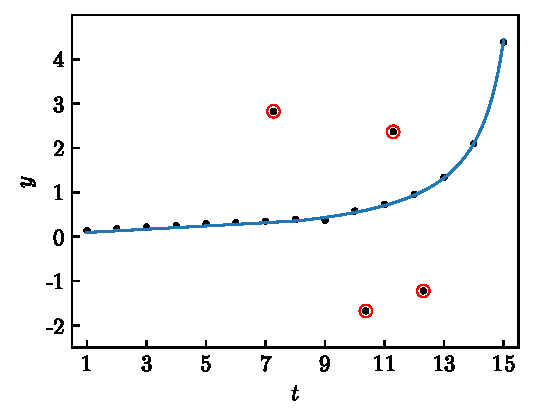
\includegraphics{images/bard_fitting.pdf}
  \caption{Bard function with four outliers: the fit returned at $o=4$ (solid
  line) follows the clean observations (dots), while the four points identified
  as outliers (circles) are discarded.}
  \label{fig:bard}
\end{figure}

As on the polynomial instance, the iteration and evaluation counts of the two
methods are comparable, and the per-instance differences carry no systematic
sign, reflecting the run-to-run variability of the multistart procedure rather
than an effect of $B$. This is perhaps surprising, since the Bard model is
nonlinear and the curvature is now informative; it is, however, consistent with
the analysis of Section~\ref{sec:complexity}, where $B$ enters only the
constants---and not the order---of the complexity bounds. Two further remarks
temper any apparent gain. First, the counts are those of the single run that
produced the reported solution and are therefore subject to the same multistart
variability. Second, the evaluation count $f\!\operatorname{cnt}$ does not
account for the extra work performed by the quasi-Newton variant at every
iteration---the assembly and spectral processing of the curvature matrix of
each active component---so the modest differences in $f\!\operatorname{cnt}$ do
not translate into a reduction in running time. In summary, on this nonlinear
instance the curvature preserves the theoretical guarantees and the solution
quality while offering no systematic computational advantage, in line with the
complexity analysis.

\begin{table}[t]
  \centering
  \begin{tabular}{c rrr rrr}
    \toprule
      & \multicolumn{3}{c}{First-order ($B=0$)}
      & \multicolumn{3}{c}{Quasi-Newton ($M=1$)} \\
    \cmidrule(lr){2-4}\cmidrule(lr){5-7}
    $o$ & $f(x^\star)$ & \#it & \#fcnt & $f(x^\star)$ & \#it & \#fcnt \\
    \midrule
    0 & 3.239e$+$00 & 24 &  94 & 3.238e$+$00 & 25 &  60 \\
    1 & 3.162e$+$00 &  7 &  27 & 3.143e$+$00 &  8 &  28 \\
    2 & 3.140e$+$00 & 13 &  53 & 3.136e$+$00 & 13 &  54 \\
    3 & 5.994e$-$01 & 15 &  58 & 6.029e$-$01 & 24 & 102 \\
    4 & 1.613e$-$03 &  7 &  15 & 2.785e$-$03 &  2 &   5 \\
    5 & 6.737e$-$04 & 58 &  62 & 4.614e$-$04 &  6 &   9 \\
    6 & 3.394e$-$05 &  4 &   9 & 4.728e$-$05 &  6 &   9 \\
    \midrule
    $\Sigma$ & & 128 & 318 & & 84 & 267 \\
    \bottomrule
  \end{tabular}
  \caption{Bard function ($m=15$, $\delta=0.1$) with four outliers at indices
  $\{3,7,11,15\}$: first-order method ($B=0$) versus the quasi-Newton variant
  ($M=1$). For each $o$, the best $f(x^\star)$ over $100$ starting points, the
  number of outer iterations (\#it) and the number of function evaluations
  (\#fcnt) of the run attaining it.}
  \label{tab:bard}
\end{table}
